 
%Juanlu: Incluyo algunos templates de diapositivas

\section{Introduction}

%%%%%%%%%%%%%%%%%%%%%%%%%%%%%%%%%%%%%%%%%%%%%%%%%%
\begin{frame}{Context}

\begin{columns}

\column{.5\textwidth}
 \begin{itemize}
  \item \textcolor{red}{Algorithm} %(a finite list of well-defined instructions for calculating a function)
  \begin{itemize}
   \item Calculus
   \item Data processing
   \item $\dots$
  \end{itemize}
 \item \textcolor{red}{Computational Intelligence}% (algorithms to solve complex real-world problems)
 \begin{itemize}
   \item Artificial neural-networks
   \item Evolutionary computation
   \item Swarm intelligence
   \begin{itemize}
     \item Particle swarm optimization
     \item \textcolor{blue}{Ant colony optimization(ACO)}
   \end{itemize}
   \item $\dots$
  \end{itemize}
 \end{itemize}
\column{.5\textwidth}

\begin{center} 
  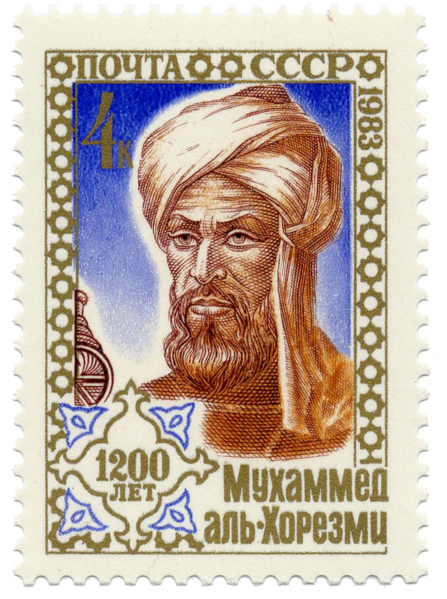
\includegraphics[width=5cm]{images/al-Khwarizmi.png} 
\end{center} 

\end{columns}

\end{frame}
%%%%%%%%%%%%%%%%%%%%%%%%%%%%%%%%%%%%%%%%%%%%%%%%%%
\note{Talk no more than 1 minute.}



%%%%%%%%%%%%%%%%%%%%%%%%%%%%%%%%%%%%%%%%%%%%%%%%%%
\begin{frame}
\frametitle{A key concept: Emergence}
\begin{columns}
\column{.6\textwidth}
 \begin{itemize}
  \item Social animals like ants cooperate and describe emergent behaviors
  \item<2-> But not only ants
 \end{itemize}
\column{.4\textwidth}
\includegraphics<1>[width=4cm]{images/al-Khwarizmi.png}
\includegraphics<2->[width=4cm]{images/al-Khwarizmi.png}
\end{columns}
\only<3>{
\begin{block}{Emergence [Wikipedia]}
Emergence is the way complex systems and patterns arise out of a multiplicity of relatively simple interactions
\end{block}
}

\end{frame}
%%%%%%%%%%%%%%%%%%%%%%%%%%%%%%%%%%%%%%%%%%%%%%%%%%
